\chapter{Project Structure}
\label{sec:projstructure}

\textit{Covered in \href{https://www.youtube.com/watch?v=fbbjnhs4nyo&list=PLjGmdnqrOKuYXiu7lgG5HW71jPEUd1XCm&index=3}{video 2 of the series}}
\vspace{6mm}

We will tour around the project and explain a little bit on how the website works. It is just a brief overview, you do not need to remember and understand every detail, the most important thing to learn is how to use them, which will be taught in later chapters.

\section{Overview}

The \texttt{app} folder contains everything you need to generate the website. The Pug files, the styles written in Less, JavaScript files, images, etc.. Then by running \texttt{npm run build}, commanding the \texttt{gulpfile.js} and \texttt{node\textunderscore modules} to work together, it translates the Pug files into HTML files, less styles into CSS files, and copies other files to the \texttt{docs} folder. The \texttt{docs} folder is the final output of the website, we can open the HTML files directly using a browser.

\section{Pug files}

Pug files are translated into HTML files, they provide the basic structure of the web page. All Pug files should be put inside \texttt{app/templates}.

\subsection*{Views}

The \texttt{app/templates/views} folder contains the content body of each page. Each Pug file in this folder would be translated to an HTML file with the same name in \texttt{docs}. As you can see, \texttt{abouts.pug} is translated into \texttt{abouts.html} while \texttt{index.pug} is translated into \texttt{index.html}. They all \texttt{extends ../layouts/default}, meaning that they follow the layout in \texttt{app/templates/layouts/default.pug}, which we will look at in a second. (Reminder: \texttt{..} means previous directory)

\subsection*{Layouts}

The \texttt{app/templates/layouts} folder contains \texttt{default.pug}. It is a template for \textbf{all} pages. It includes common elements like the page title, the styles import, the navbar and the footer. 

Then under \texttt{block content} in line 55, each page in the \texttt{views} folder inserts their own content under this block. Knowing the exact syntax is not required.

\subsection*{Partials}

The navbar and footer are separated from the \texttt{default.pug} to make it cleaner. They are put in the \texttt{app/templates/partials} folder, and got included in \texttt{default.pug} in lines 38 and 61 respectively.

\begin{figure}[h]
\centering
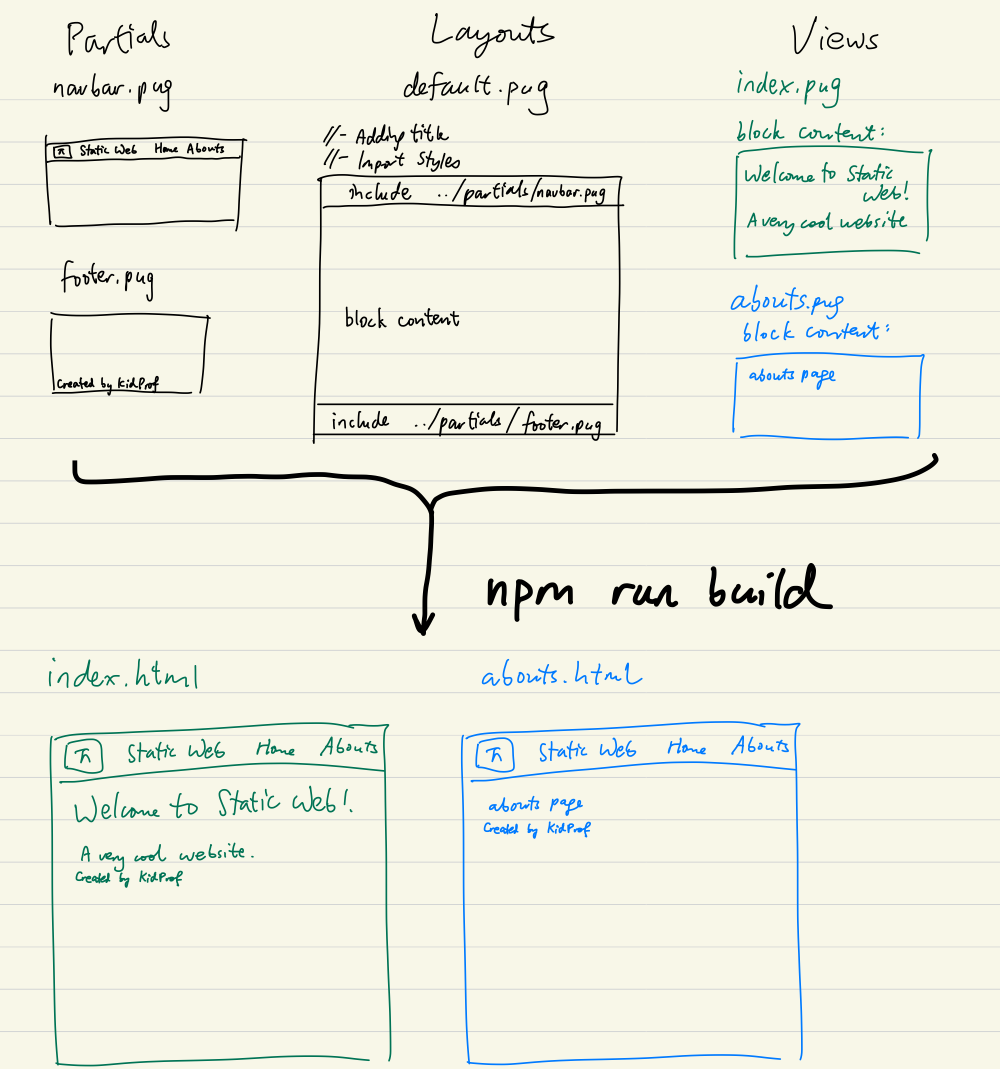
\includegraphics[width=13cm]{images/ch4-puglayouts.png}
\caption{Overview on how Pug files are translated}
\end{figure}

\section{Styling files}

We will be using less files for styling in place for CSS, which are placed under \texttt{app/styles}. The \texttt{site.less} file includes all files under the \texttt{app/styles/site} folder, \textbf{remember to add the file to \texttt{site.less} whenever you are creating a new less file}. 

The files under the \texttt{site} folder should be where you write the styles. By convention, \texttt{layout.less} should contain styles that is used in all/ multiple pages; \texttt{variables.less} should contain all variables; and other files should contain styles that is only used in the page with the same name as the style file. This is just a convention but not a rule, there is nothing to enforce it until \hyperref[sec:confinestyles]{chapter 8}.

When we run \texttt{npm run build}, the styles got translated into CSS and put into a single file \texttt{docs/styles/site.css}. The stylesheet is imported into all HTML files in line 18 of \texttt{layout.pug}.

\section{Generated Files}

We kept mentioning \texttt{npm run build} as if it is some sort of magic, now it's time to look a little bit closer.

\subsection{\texttt{package.json}}

This file contains basic information about our project (change the name and description if you like). What is more important is the dependencies and the devDependencies, it tells what \texttt{npm}\footnote{stands for Node Package Manager} what libraries you need to run this project, it is written by me, so all you have to do is to run \texttt{npm install} (what you did already in chapter 1), and it knows what to install for you, without the need of you specifying what to install.

Also the scripts section specifies what will be run on \texttt{npm run ...}, from the line \texttt{"build": "gulp build"}, it means the command \texttt{gulp build} will be run when we run \texttt{npm run build}. More in the \hyperref[sec:gulpfile]{later subsection}.

\begin{lstlisting}[language=]
{
  "name": "static-web-sandbox",
  "version": "2.0.0",
  "description": "A very cool website.",
  "dependencies": {
    "gulp": "^4.0.0"
  },
  "devDependencies": {
    "@babel/core": "^7.2.0",
    "@babel/preset-env": "^7.2.0",
    "gulp-babel": "^8.0.0",
    "gulp-changed": "^3.2.0",
    "gulp-eslint": "^5.0.0",
    "gulp-imagemin": "^5.0.3",
    "gulp-less": "^4.0.1",
    "gulp-pug": "^4.0.1",
    "less-plugin-autoprefix": "^2.0.0"
  },
  "scripts": {
    "test": "echo \"Error: no test specified\" && exit 1",
    "build": "gulp build"
  },
  "license": "ISC"
}
\end{lstlisting}

\subsection{\texttt{node\textunderscore modules} folder}

This folder is automatically generated when you run \texttt{npm install}.\footnote{To verify, remove this folder using \texttt{rm -rf node\textunderscore modules} and run \texttt{npm install} again.} It contains the library files you need to run this project, the project would not run without this folder. \textit{You do not need to edit this file at all.}

\subsection{\texttt{package-lock.json}}

This is an automatically generated file, it outlines in detail which version of the dependencies are installed. It automatically updates when you run \texttt{npm install}. \textit{You do not need to edit this file at all.}

\subsection{\texttt{gulpfile.js}}
\label{sec:gulpfile}

This file is responsible for the translation process. As you can see, the task \texttt{pug} translates each \texttt{.pug} file under \texttt{app/templates/views} to HTML files and put them under \texttt{docs}. Similar translation happens for less files. The JavaScript files, images and fonts are copied to the \texttt{docs} folder.

Finally, the task \texttt{build} runs all the above commands. Therefore, \texttt{gulp build} does what is is supposed to do. \textit{You do not need to edit this file at all.}

\begin{lstlisting}[language=JavaScript]
// gulpfile.js
...

//pug to html conversion
gulp.task('pug', function(){
  return gulp.src("app/templates/views/*.pug")
  .pipe(changed("docs/")) //pipe files only if changed 
  .pipe(pug({pretty:true})) //pug to html
  .pipe(gulp.dest('docs/'));
});

//less to css conversion
gulp.task('styling', function(){
  return gulp.src("app/styles/site.less")
  .pipe(changed("docs/styles")) //pipe files only if changed 
  .pipe(less({
    plugins: [autoprefix]
  })) //less to css
  .pipe(gulp.dest('docs/styles'));
});

gulp.task('js',function(){ ... });
gulp.task('imagecopy',function(){ ... });
gulp.task('fontcopy',function(){ ... });

gulp.task('build',gulp.series('js','pug','styling','imagecopy','fontcopy'));

\end{lstlisting}

\subsection{\texttt{docs} folder}

This folder is automatically generated when you run \texttt{run build}.\footnote{To verify, remove this folder using \texttt{rm -rf docs} and run \texttt{npm run build} again.} It is the output folder of the whole project, you can directly open the HTML files inside the folder. You should upload this folder to web servers in order to host it.
\textit{You do not need to edit this file at all.}

\subsection{\texttt{.gitignore}}
\label{sec:gitignore}

Because the \texttt{node\textunderscore modules} folder and the \texttt{docs} folder can be automatically generated on your own local machine. There is no need to put these onto GitHub. The \texttt{.gitignore} file lets you state the files and folders that you do not want to push to GitHub. It includes the two folders I have mentioned, and some others that are out of our scope.

\section{Other files}

\subsection{\texttt{README.md}}
\label{sec:readme}

This file serves as a documentation. It will be displayed on GitHub. You should write a description of your project, and how to install and use it in here. The syntax is a bit weird, refer \href{https://docs.github.com/en/get-started/writing-on-github/getting-started-with-writing-and-formatting-on-github/basic-writing-and-formatting-syntax}{here}\footnote{Link: \url{https://docs.github.com/en/get-started/writing-on-github/getting-started-with-writing-and-formatting-on-github/basic-writing-and-formatting-syntax}} if you want to write your own README.

\subsection{\texttt{.eslintrc}}

\textit{Of less importance}

This file stores the JavaScript settings and version we are using, so as to check for syntax errors when copying JavaScript files from \texttt{app} to \texttt{docs}. \textit{You do not need to edit this file at all.}